\documentclass[a4paper, 11pt]{article}
\usepackage[utf8]{inputenc} 
\usepackage[T1]{fontenc}
\usepackage{graphicx}
\usepackage[french]{babel}
\usepackage[labelfont=bf]{caption}
\usepackage{subcaption}
\usepackage{rotate}
\usepackage{float}
\usepackage{url}
\usepackage{hyperref}
\usepackage{setspace}
\usepackage{titling}

\captionsetup{labelfont=bf}

\pretitle{%
  \begin{center}
  \LARGE
  
\includegraphics[scale=0.8]{LogoUnicaen}\\[\bigskipamount]
}
\posttitle{\end{center}}

\title {Rapport de soutenance du projet}
\author {Daniel MURRAY, Léo MALUBIER, Martin AUBLET, Hasti KHAYAMI}

\begin {document}

\maketitle

\newpage

\section{Tableau de Contenu}

\tableofcontents

\newpage

\section{Manuel d'utilisation}

\subsection{Lancement du programme}

\begin{itemize}

\item{Windows:}
\begin{itemize}

\item{Naviguer dans le dossier "src", et double-cliquer sur le fichier "wargame.py" se-trouvant à la racine du dossier pour lancer le simulateur.}

\end{itemize}
\item{Linux:}
\begin{itemize}

\item{Ouvré un terminal dans la racine du dossier, et saisir le suivant:}
\item{python src/wargame.py}

\end{itemize}

\end{itemize}


\subsection{Utilisation}

Lors du lancement du programme, 3 options sont proposés.

\begin{itemize}

\item{"Simuler une bataille" - Simule un combat singulier entre deux armées à une vitesse ralenti, pour pouvoir visualiser les statistiques d'un combat tour-par-tour.}
\item{"Optimiser une armée" - Générer une armée avec un pourcentage de victoire maximisé, basé sur un plateau de jeu et des simulations de combat.}
\item{"Quitter" - Fermer le programme.}

\end{itemize}

\begin{figure}[!htbp]

\begin{center}

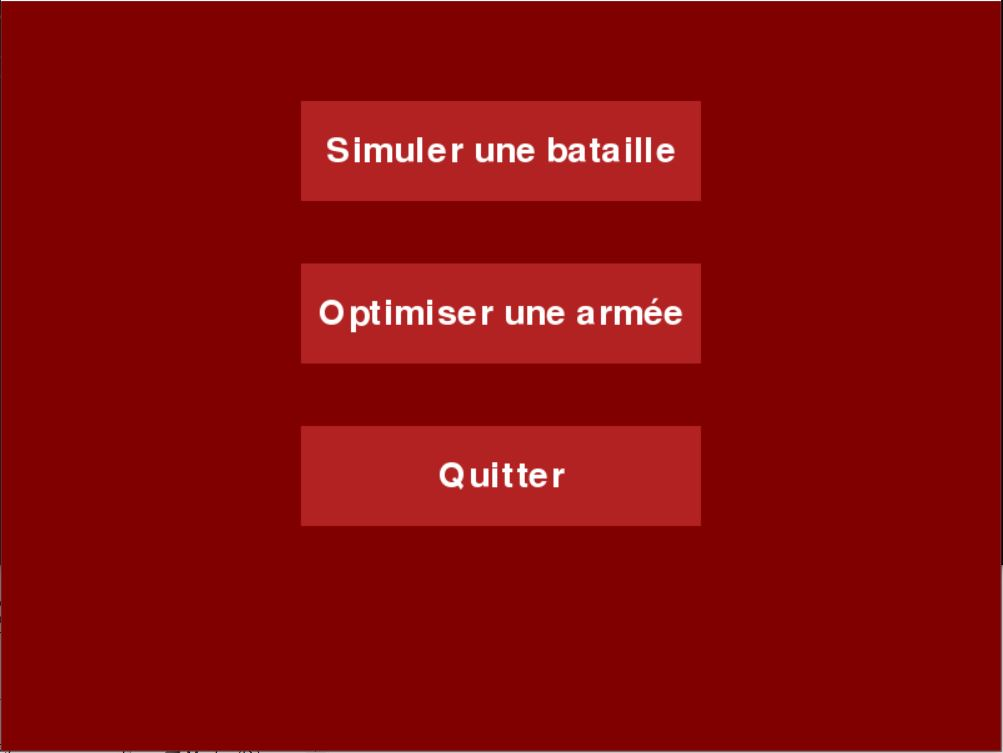
\includegraphics[scale=0.3]{Menu}
\caption{Le menu principale du programme.}

\end{center}

\end{figure}

\subsubsection{Simuler une bataille}

Dans cet section du programme, on simule un combat singulier, entre deux armées sur un plateau de jeu, à une vitesse ralenti, pour pouvoir visualiser les statistiques d'un combat tour-par-tour
Quand cet section est ouvert, le programme commence par générer un plateau de jeu. Quand ceci est fait, le programme attend que l'utilisateur clique sur la barre d'espace pour commencer la simulation.
Une simulation est alors effectué, un tour à la fois. A la fin de chaque tour, plusieurs données sont visibles et accessibles à l'utilisateur, pour permettre la visualisation et analysé les résultat. \\
A la fin de la simulation, les résultats de la bataille sont affichés.

\begin{figure}[!htbp]

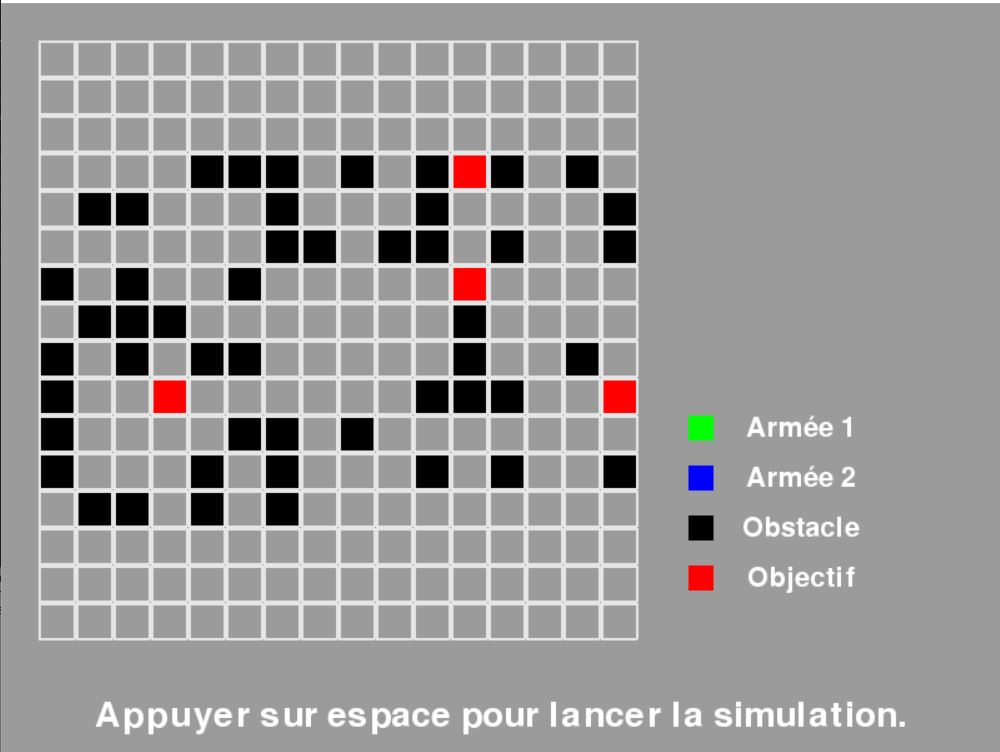
\includegraphics[scale=0.3]{Simulation-Start}
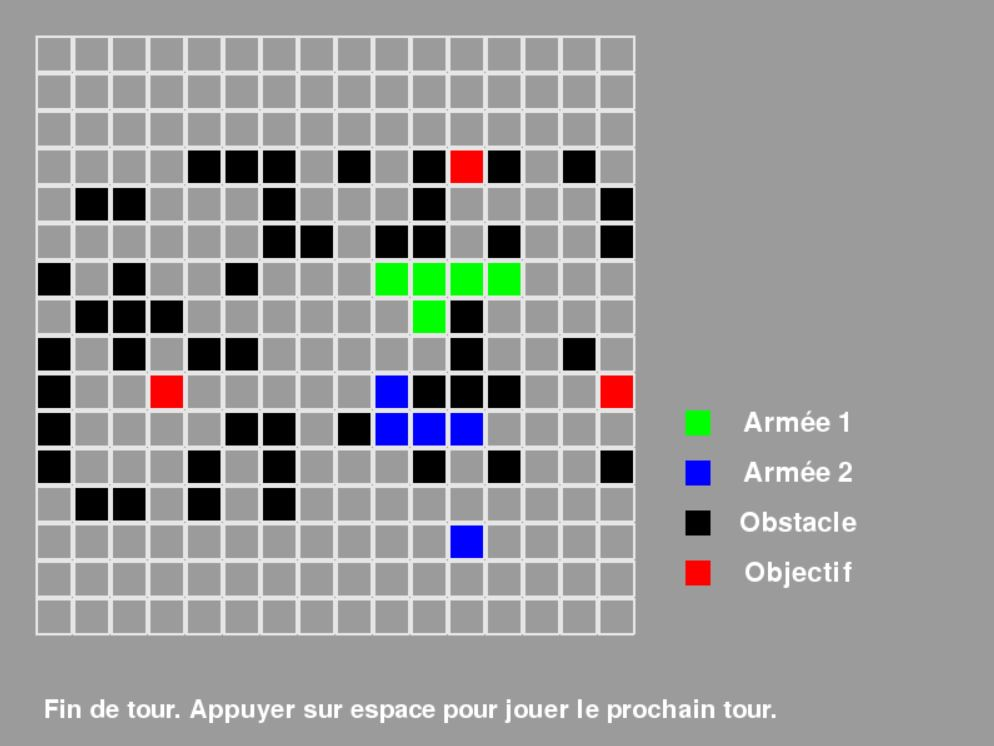
\includegraphics[scale=0.3]{Simulation-InProgress}

\caption{Captures d'écran d'une simulation.}

\end{figure}

\subsubsection{Optimiser une armée}

Dans cet section, on lance plusieurs simulations avec différents armées générés aléatoirement, pour optimiser et pouvoir générer une armée qui sera la meilleur.
Ce processus est largement optimisé grâce à des algorithmes et fonctions, qui nécessite très peu d'action de la part de l'utilisateur. \\
A la fin du processus, le programme affiche la meilleur armée. 
On peux voir les statistique dans la console, et l'armée qui a remporté. 


\begin{figure}

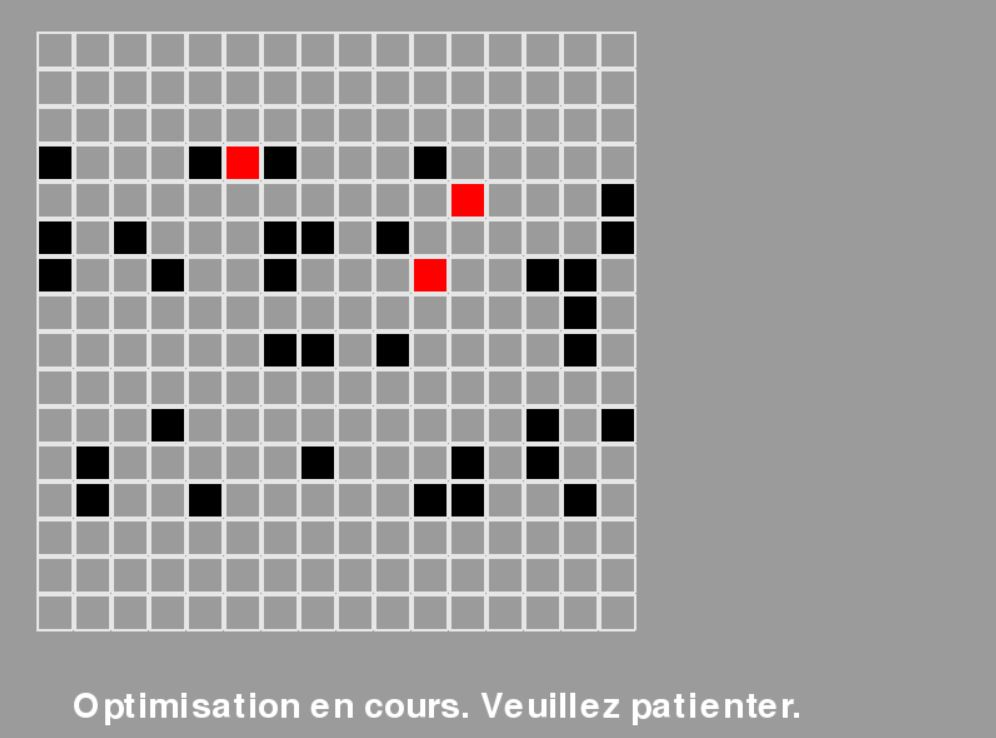
\includegraphics[scale=0.3]{Optimisation-InProgress}
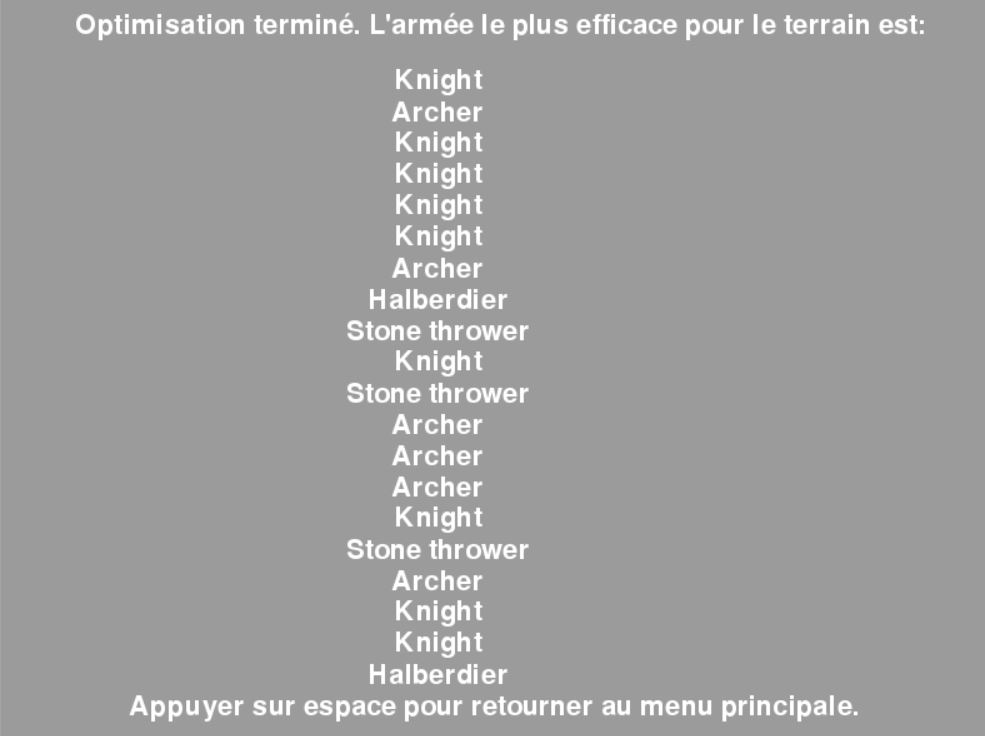
\includegraphics[scale=0.3]{Optimisation-Finished}

\caption{Captures d'écran d'une optimisation.}

\end{figure}

\section{Organisation}

\subsection{Répartition des tâches}

\begin{center}
\begin{tabular}{ |c|c| } 
 \hline
 Codage des objets et modèles,visualisation simulation & Daniel MURRAY \\ 
 Combat, optimisation, traitement des données simulation & Léo MALUBIER \\ 
 Interface graphique, sprites & Martin AUBLET \\
 Codage graphique menu, PyGame  & Hasti KHAYAMI  \\
 \hline
\end{tabular}
\end{center}

\subsection{Ecriture des fichiers}

\begin{center}
\begin{tabular}{ |c|c| } 
 \hline
 modeles.py,optimisateur.py & Daniel MURRAY \\ 
 combat.py,combat.py & Léo MALUBIER \\ 
 mainmenu.py, unites.py & Martin AUBLET \\
 mainmenu.py, modeles.py  & Hasti KHAYAMI  \\
 \hline
\end{tabular}
\end{center}

\subsection{Contact}

\begin{center}
\begin{tabular}{ |c|c| } 
 \hline
 Daniel MURRAY & 07 52 05 17 13 \\ 
 Léo MALUBIER & 06 38 01 14 29 \\ 
 Martin AUBLET & \\
  Hasti KHAYAMI & 07 79 46 62 24 \\
 \hline
\end{tabular}
\end{center}

\section{Objectifs du projet}

\subsection{Description du concept}

\begin {center}
Le but de ce projet est de réalisé un simulateur et optimisateur de "wargame", qui permet de construire une armée qui aura un pourcentage maximum de victoire, en relation du terrain sur le plateau du jeu, et contre un autre armée quelconque.
\end {center}

\subsection{Les éléments existants}

La pratique du "wargame" est principalement appliquée par le militaire pour des entraînements stratégiques, mais il existe aussi une vaste variété de jeux de société qui ont pour but de recréer cet expérience de manière amusant. \\

Des différentes variantes existent avec leurs propres règles et procédures. Pour maximiser la simplicité et la compréhension du côtés programme et utilisateur, nous avons choisi d'utilisé un l'ensemble de règles trouvés dans \href{https://onepagerules.com/portfolio/grimdark-future-firefight/}{"Grimdark Future: Firefight"} comme base. Nous avons aussi modifié ou supprimé certains règles et procédures ci-trouvant pour gardé la simplicité du déroulement. \\

Notre langage de programmation choisi est Python, pour ses capacités d'écriture simple et sa robustesse. De plus, nous intégrons aussi le bibliothèque "PyGame", qui rend possible des fonctions et méthodes pour l'affichage graphique.Un module math est aussi utilisé, et deepcopy. \\

\subsection{Les éléments à développer}

Pour pouvoir créer un optimiseur de wargame, notre but est divisé en quatre taches: \\

\begin{enumerate}

\item Recréer l'ensemble des règles choisis de wargame dans python.
\item Simuler le combat entre les armés en respectant l'ensemble de règles choisis.
\item Développer un optimiseur qui générera une armée efficace en relation avec le système de combats lors de l'étape précédente.
\item Afficher le tout dans un interface graphique simple et facile à comprendre et utiliser.

\end{enumerate}

\begin{figure}[h]

	\centering
	
\includegraphics[scale=0.4]{grimdark}
	\caption{Logo de Grimdark Future: Firefight.}

	
\includegraphics[scale=0.4]{Pygame}
	\caption{Logo de PyGame.}
\end{figure}

\newpage

\section{Fonctionnalités implémentées}

\subsection{Description des fonctionnalités}

Notre projet peut être divisé en quatre parties principales. Chaque résultat d'une partie peut contribuer ou fournir les variables nécessaires pour une autre. \\

Le simulateur simule des combats. Si nous souhaitons simuler le combat entre 15 armées, on effectue 25*26 combats. On prend une armée qui va combattre les 25 autres armées, puis repeter ceci 26 fois pour tester les autres armées. Chacune des armées à ses propres unités crées à partir du format trouvé dans l'ensemble des règles, sur un plateau de jeu généré aléatoirement avec des objectifs et des obstacles. \\

Chaque résultat de chaque combat est enregistré, et l'armée avec le plus de victoire est considéré comme gagnant, ou pourra passer a l'étape suivant qui est l'optimisation.\\

L’intégralité de notre programme sera encadré par une interface graphique, à travers les fonctions d'affichage et rendus grâce à PyGame. \\

\subsection{Organisation du projet}

Notre groupe de projet est constitué de 4 personnes. Nous nous somme donc répartis les taches que nous voulions réalisé.\\

\begin{itemize}

\item Une personne code et transforme l'ensemble de règles utilisés en fonctions, classes et objets dans Python. \\
\item Un personne interprètent les instructions et règles pour concevoir un arbre de décision pris par l'ordinateur, les transforment en pseudo-code/algorithmes, puis ensuite le traduit et écrit en language de programmation. \\

\item Une personne développe une système d'optimisation pour pouvoir gérer les résultats des combats simulés dans le programme, et ensuite analyse et développe une armée avec des taux maximisé. \\

\item Une personne développe un système de combat qui sera utilisé lors de la simulation. Elle prendra en charge plusieurs fonctions de gestion de variables, attaque et défense, les points de vie d'une unité... \\

\item Une personne prend en charge les graphiques nécessaires. Ils créent et dessinent tous les sprites et images nécessaires, ensuite ils développe un système pour pouvoir gérer l'affichage graphique, et faire afficher les sprites et objets nécessaires. \\

\end{itemize}

\begin{figure}[h]

	\centering
	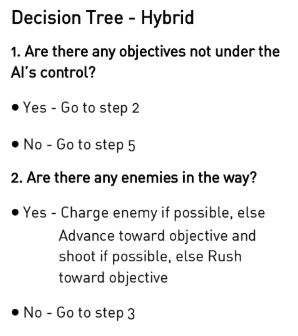
\includegraphics[scale=0.6]{treepreview}
	\caption{Un extrait de l'arbre de décision prise par les armés controllés par l'ordinateur. Cet arbre sera ensuite traduit en langage de programmation.}

\end{figure}

\newpage

\section{Elements techniques}

\subsection{Algorithmes}

\subsubsection{Génération du plateau de jeu}

Avant de pouvoir se lancer dans un combat entre deux armées, il est nécessaire de créer un plateau de jeu, où la simulation pourra se dérouler. Ce plateau sera constitué d'une grille 16*16, pour un totale de 256 cases. Le plateau de jeu contiendra aussi des objectifs, que les armées doivent capturer et défendre, et des obstacles, ou les armées ne peuvent pas se déplacer directement dessus, mais ils peuvent néanmoins les utiliser comme protection contre les attaques. \\

Pour générer notre plateau de façon aléatoire, nous suivons l'algorithme suivant:

\begin{itemize}

\item Créer une grille vide avec 16 lignes et 16 colonnes.
\item Choisir une nombre aléatoire entre 10 et 15, ce nombre correspondra au nombre d'obstacles qui sera mis sur le plateau.
\item Choisir une nombre aléatoire entre 1 et 3, et lui ajouter 2 - ce nombre correspondra au nombre d'objectifs qui sera mis sur le plateau.
\item Itérer à travers chaque case dans les colonnes de la grille, et génerer une nombre aléatoire. Si ce nombre se trouve dans un seuil, cet case sera un objectif ou un obstacle.
\item Répéter l'étape précédant jusqu’à ce que le nombre d'objectifs et d'obstacles définis est atteint.
\item Effacer les trois premiers et trois derniers lignes de la grille - ces espaces seront utilisés pour le déploiement d'armée, elles doivent être alors vides pour que les armées puissent se déployer sans problème.

\end{itemize}


\begin{figure}[!htbp]

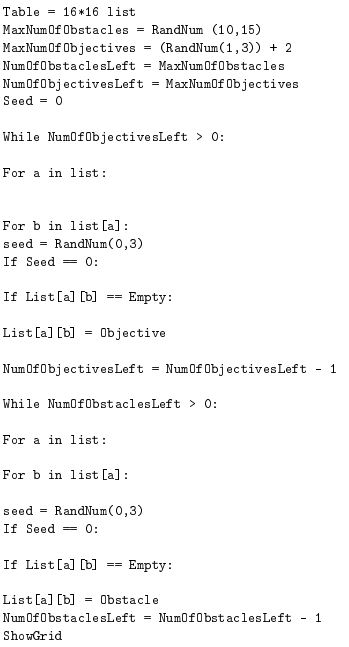
\includegraphics{PseudoCode-Terrain}

\caption{L'algorithme transformé en pseudo-code.}

\end{figure}

\begin{figure}[!htbp]

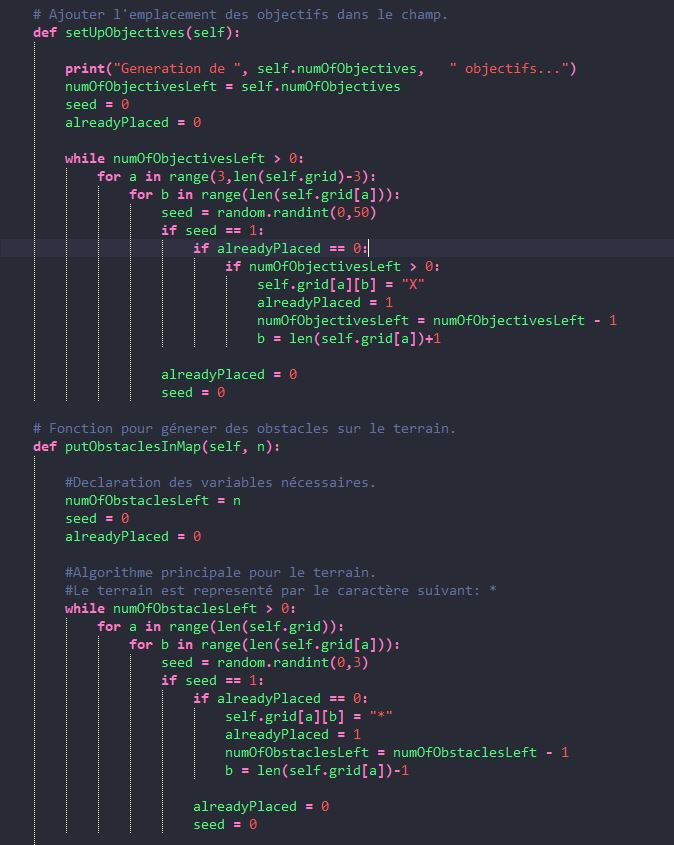
\includegraphics[scale=0.6]{Python-Terrain}

\caption{L'algorithme transformé en langage Python.}

\end{figure}

\subsubsection{Arbre de décision des unités}

Lors des combats entre chaque armée, l'ordinateur doit calculer quel décision prendre - se déplacer, attaquer une autre unité, etc. On appelle ceci "arbre de décision".
Il existe déjà un arbre de décision dans les documents des ensembles de règles (voir Figure n.3). \\

En général, l'algorithme pour l'arbre de décision (fonction computeOptions fichier modeles.py )est défini par le ceci:

\begin{itemize}

\item Regarder s'il y a des objectifs non contrôles. Si oui, avancer vers l'objectif, et attaquer un ennemi si possible.
\item Si non, analyser s'il y aura des ennemis en portée si l'unité avance. Si oui, avancer et attaquer l'ennemi. Si non, charger dans la direction de l'ennemi.
\item Répéter les étapes précédentes pour tous les unités dans une armée.

\end{itemize}

Chaque partie de l'algorithme aura un sous-algorithme, qu'on expliquera en détail plus tard.

\subsubsection{Boucle de jeu}

Notre boucle de jeu est un des algorithmes le plus important dans notre programme( fonction BestArmies fichier combat.py), puisque c'est elle qui gère la plupart des évènements, et sert à faire la gestion entre tous les autres sous-composantes (menus, fonctions, classes, objets...).
Lors du lancement d'un simulation de combat, la boucle de jeu est mise en fonction. \\ \\

En général, le boucle de jeu suit l'algorithme suivant: \\


\begin{itemize}

\item Générer le plateau du jeu.
\item Appelle la création d'un certain nombre d'armées aléatoire.
\item On prend une armée, et on la fait combattre toutes les autres. (On prend l'armée qui va combattre toutes les autre, on l’envoie dans la fonction boucle qui va poursuivre l'attaque tant qu'une des deux armées n'est pas battue.) Renvoyer l'armée victorieuse.   
\item Dans le combat, on va simuler une lancer de pièce pour décider quel armée pourra déployer ses unités sur le plateau en premier.
\item Déployer les armées sur le plateau.
\item Pendant qu'il y a au moins une unité de vivant dans une armée, simuler l'arbre de décision pour chaque unité dans une armée, le déplacer sur le plateau, et, si disponible, faire appel aux fonctions de combat.
\item Quand il n'y a plus d'unités de vivant dans une armée, terminer la boucle, puis passer au test de l'armée suivante.

\end{itemize}


\begin{figure}[!htbp]

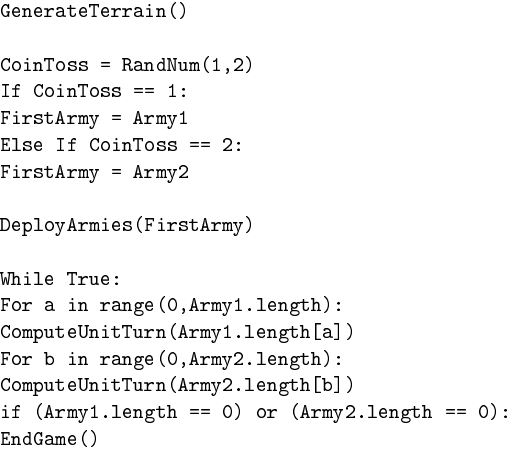
\includegraphics[scale=0.5]{PseudoCode-Boucle}

\caption{Le boucle de jeu transformé en pseudo-code.}

\end{figure}

\begin{figure}[!htbp]

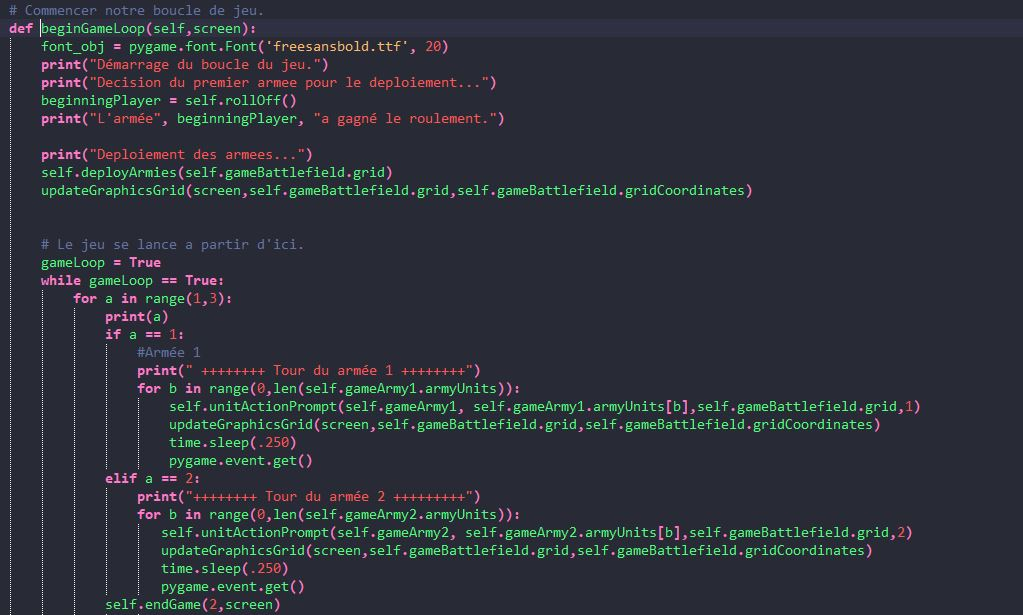
\includegraphics[scale=0.4]{Python-Boucle}

\caption{Un extrait du boucle de jeu transformé en langage Python.}

\end{figure}

\subsubsection{Optimisation d'armée}

Le simulateur de combat est le premier des parties majeurs de notre programme; l'optimisateur d'armée étant le deuxième. Elle sert à pouvoir générer une armée à partir d'un plateau de jeu, et des résultats de plusieurs combats simulés entre différents armées.
Le résultat est une armée, qui possèdera un taux de victoire plus élevé. \\ \\

L'optimisation d'armées suit l'algorithme suivant:

\begin{itemize}

\item Une armée a été choisis comme étant la plus forte (fonction BestArmies).
\item On passe par la fonction CalculStat qui permet de comparer les statistiques des deux armées les plus faible et les deux armées les plus puissantes, pour savoir quelle est le point d'écart le plus élevé entre les armé perdantes et gagnants (on compare la vie, le coût l'agilité, le mouvement et la porté) et on compte combien de chaque unité, il y a dans les armées (des chevaliers, des archers, etc).
\item Ensuite, on a un arbre de décision qui permet de modifier les armées, selon les condition que l'on a déduit grâce au calcule de la fonction CalculStat. 
Ainsi,on définit les point a maximiser (agilité par exemple) et on applique des changements. Cependant, on vérifie que l’ensemble des unités que l'on change ne contiens pas un nombre significatif pour l'armé d'unité correspondant au changement. (ici défini par le nombre total d'unité fois 1/5, ce qui est généralement autour de 4.
\item Une simulation va nous permettre de savoir si les modification apporté rend meilleur l'armée ou non. Pour cela on l'affrone x fois l'armé la plus faible, et on fait de même avec sa version précédente. Puis l'on compare qui a le plus haut taux de victoire en pourcentage.
\item Enfin on affiche l'armée avec le plus haut taux de victoire suite au modifications. Si l'armée modifié a un taux de réussite plus haut que l'armé de départ, alors elle est meilleur. Au contraire, elle peux être moins bonne, ce qui signifie que la meilleur armée était celle de départ et que l'on ne peux pas l'améliorer.  


\end{itemize}


\subsection{Structures de données}

La majorité des composantes qui font partie d'un wargame (exemples: le plateau du jeu, chaque unité d'une armée, etc) peuvent être répliqués sur Python avec la notion des "objets" dans Python. Chaque objet aura la possibilité de porter ses propres données, variables et fonctions. De plus, chaque objet peut être "instantané" pour pouvoir en créer plusieurs objets d'une même classe. Ceci est très utile pour la gestion de plusieurs éléments en même temps. (Exemple: tous les unités dans une armée sont tous des objets) \\

Dans cet section, nous entrons en détail dans le structure de quelque objets critiques dans notre programme.

\subsubsection{Les armées}

Chaque armée peut être considéré comme objet Python. Pour faciliter la compréhension et gestion de chaque unité dans notre armée, tous les objets unité seront enregistré dans une liste, qui sera ensuite stocké par notre objet armée. Lors du création de l'armée, l'objet fait appel à un fonction qui génère des objets pour les unités aléatoire, puis les stocke dans une liste dans notre objet.  \\ \\


\begin{itemize}

\item{maxPoints: Le cout maximum que tous les unités d'un armée peuvent y être.}
\item{maxArmyUnits: Le nombre maximum d'unités dont l'armée peut y être.}
\item{armyUnits: Une liste qui stockera tous les objets Unité lors du création de l'armée.}

\end{itemize}

\subsubsection{Les unités}

Chaque unité d'une armée a plusieurs variables qu'on peut facilement manipuler lors de la simulation de combat. Lors de l'initialisation de cet objet, certaines  variables sont passés en argument, pour structurer l’objet (la santé, endroit sur le plateau du jeu, etc...) \\ \\

Variables: \\

\begin{itemize}

\item{Health: Le points de vies de l'unité.}
\item{Wounds: Le nombre de blessures dont l'unité porte. Si cet variable est égale ou supérieure a Health, l'unité est alors supprimé de l'armée et du plateau du jeu.}
\item{Location: Les coordonnées x et y de l'unité sur le plateau du jeu. Elle est représente comme une liste [x,y].}
\item{Name: Le type de l'unité. Representé avec un String.}
\item{Cost: Le cout de l'unité.}

\end{itemize}

\subsubsection{Le système de jeu}

Le système utilisé pour suivre et gérer chaque simulation est un des composants le plus importants dans notre programme (voir partie 4.1.3). Il dirige la boucle principale de notre programme, et sert à faire la gestion entre tous les autres sous-composantes (menus, fonctions, classes, objets...).
Cet objet est rempli de plusieurs fonctions et variables nécessaires pour le déroulement correct de la programme. \\ \\

\begin{itemize}

\item{test}

\end{itemize}

\subsection{Bibliothèques}

\subsubsection{PyGame}

Pour permettre une visualisation graphique du simulation et l'optimisation, nous aurons besoin d'une bibliothèque Python qui permet l'utilisation des fonctions liées à l'affichage d'une interface graphique interactif.
Pour satisfaire ces besoin, nous utiliserons la bibliothèque PyGame, qui donne l'accès aux fonctions pour manipuler des aspects graphiques de notre programme.

\newpage

\section{Architecture du projet}

\subsubsection{Fichiers du projet}

Pour permettre une organisation plus nette et plus claire de notre projet, chaque partie d'une programme (simulateur, menu principale, etc..), et ses fonctions correspondants seront reparti, chacun dans son propre fichier. Exemple: Un fichier pour les fonctions du menu principale... \\

Notre fichiers principales sont les suivants:

\begin{itemize}

\item{combat.py: Fonctions de combat utilisés lors du simulation.(permet de faire l’optimisation }
\item{mainmenu.py: Fonctions pour le menu principale.}
\item{modeles.py: Fonctions principales du programme, boucle de programme, etc. Elle contient aussi tous les classes et fonctions principales.}
\item{optimisateur.py: Fonctions pour l'optimisation d'armée.(du menu interactif)}
\item{unites.py: Classes des unités utilisés lors du simulation.}
\item{wargame.py: Le ficher exécuté pour lancer le simulateur; le point d'entrée du programme.}

\end{itemize}

\subsubsection{Aborescence du fichier}

Pour permettre la gestion simplifié du projet, chaque dossier, sous-dossier et fichier de notre programme doit porter un nom qui est en relation avec son contenu. De plus, le nombre de dossiers et sous dossiers devront être limités, pour éviter de partir dans tous les directions pour faire la recherche d'un ficher spécifique. \\
Pour pouvoir respecter ces besoins, nous avons construit le dossier du projet du manière suivante:

\begin{itemize}

\item{Le racine du dossier contiendra deux dossiers, appelés "src" et "docs" respectivement.}
\item{Le dossier src contiendra tous nos fichiers Python (.py).}
\item{Le dossier docs contiendra tous les fichier liées au rapport LaTex, pour pouvoir le générer.}
\item{Un dossier caché appelé ".svn" est parfois visible dans la racine du dossier. Cet dossier sert au comme paramètrage pour le répositoire en ligne.}
\item{Un fichier texte appelé "README.txt" est aussi disponible dans la racine du dossier.}

\end{itemize}

\begin{figure}

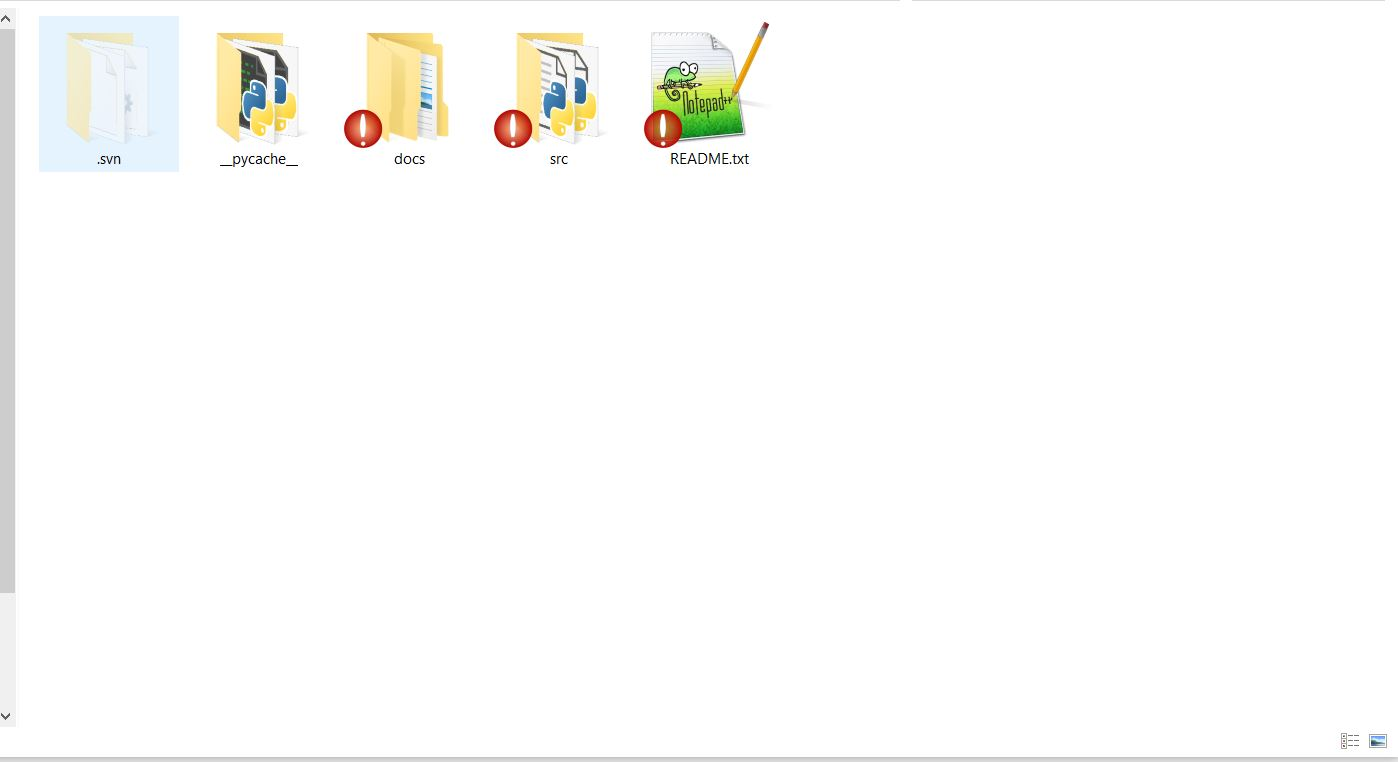
\includegraphics[scale=0.5]{FolderRoot}

\caption{Une capture d'écran du racine du dossier.}

\end{figure}

\newpage

\section{Conclusion}

Grâce aux algorithmes et fonctions implémentes dans notre projet, les objectifs principales de notre projet ont été atteints sans des soucis majeurs. Il y a certains éléments de la programme que nous avons souhaités réaliser mieux (exemple: les aspects graphiques), mais en cause du COVID-19 nous forcant à travailler à notre foyers, nous n'avions pas pu récuperer certains fichiers stockés sur les ordinateurs de l'université. A la suite de ceci, nous étions contraints de réaliser certains graphiques d'une manière moins précis. 
Le temps d’exécution de la boucle principale, et de la simulation nous contrains à devoir réduire le nombre d'armées. Nous en avons mis 26 armées, en raison que une des nombres les plus élevées, qui prend le moins de temps à avoir un résultat. Nous devons faire combattre 25*26 armées, soit 650 simulations de comba,t plus une moyenne de 19 unités par armée, soit plus de 12 350 interaction sans compter la partie optimisation qui prend moins de temps. 
L'optimisation se basant sur des statistiques, l'algorithme d'optimisation n'est pas sur a 100\% d'avoir une optimisation réussis de l'armée. 
Nous considérons que, si une armée optimisé n'a pas passé le test de réussite, alors l'armée la plus puissante reste celle de base et sur l'échantillon d'armée, elle est la plus puissante.\\



\newpage

\end{document}